%!TEX program = xelatex
\documentclass[letterpaper,11pt]{ctexart}
\usepackage{natbib}
\bibliographystyle{unsrtnat}
\usepackage{amsmath}  
\usepackage{graphicx} 
\usepackage[margin=1in,letterpaper]{geometry}
\usepackage{libertine}
\usepackage[final]{hyperref}
\hypersetup{
	colorlinks=true,      
	linkcolor=blue,       
	citecolor=blue,        
	filecolor=magenta,
	urlcolor=blue         
}
\usepackage{xeCJK}
\usepackage{titlesec}

\titleformat{\section}{\flushleft\bfseries\Large}{\thesection}{1em}{}

\linespread{1.5}

\begin{document}

\title{FORT:一种无限流动性的DeFi开发及应用系统}
\author{Zaugust \\ James Zhao}
\date{2021年9月9日}
\maketitle


链上应用的关键是流动性,为了解决流动性问题,之前的去中心化金融(DeFi)尝试了传统观念的订单簿(Orderbook)和自动做市商(AMM)模型,但这些模型都不是理想的解决方案,并且无法将所有金融服务纳入到同一个协议并共用同一个流动性,造成资源的浪费和效能的低下。
本文提出一种新的模型:FORT协议,这种协议创造了折现计算机及链上货币单位的概念,系统解决了所有DeFi的流动性及统一性问题,可用于一切金融产品及链外活动的经济关系锁定。

\section{DeFi的历史}

DeFi是区块链领域发展最为迅猛并找到真实需求的应用,他们产生的历史可以追溯到早期基于Orderbook的链上交易,以及点对点的借贷,这些应用在2017年左右获得一定的关注,但由于链上撮合成本极高、去中心化预言机缺失,这一类项目并没有发展起来。
反而是基于AMM机制的Uniswap和基于资金池和资产价格的借贷协议Compound、MakerDAO等迅速崛起,并引领了DeFi的浪潮,因为这一类项目更好的解决了DeFi的根本矛盾:链上流动性匮乏。

但无论AMM也好,资金池也好,其解决流动性问题的方法都是以牺牲了卖方的灵活性为代价的,即卖方需要把自己的交易策略固定下来并承担外部市场的波动,一旦价格有利于卖方,买方可能选择退出交易,一旦存在套利,买方便蜂拥而至,整个过程卖方没有任何选择权,只能寄希望于挖矿的补贴和大数规则下的佣金或利率均衡。
这种不对称的设计虽说暂时缓解了链上流动性的匮乏,但长期来看存在以下问题:首先是资金的大量占用导致资源浪费,链上如此众多的锁仓量(TVL)却只支持了少量的交易,而且大部分TVL还是冲着流动性挖矿而来;其次是核心变量,如价格、利率等和池子的规模有关,一方面容易被套利,另一方面在池子规模不够的情况下,交易和借贷很难开展。而且,不同产品的TVL不能共用,导致所谓的组合行也只是形式上的组合,而不是流动性的共享。

这种牺牲一方选择权而创造出来的流动性,并不是去中心化架构下的完美思路。
与其让卖方做出不对称的牺牲,不如将这种不对称彻底抹除——系统只允许存在完全对称的买方,卖方为系统本身。
这一思想符合区块链去中心化博弈的精神:大家都是处于同一个位置和算法进行博弈,无论是比特币,以太坊都是如此。
每个参与者,只需要向系统支付对价的系统代币,就能得到想要的金融产品,而金融产品的收益由系统代币增发结算。
这一思想将我们从传统的金融交易模型里解放出来,可以形成一个新的金融范式,而且保证DeFi不仅仅是具备可组合性,而是等价于同一框架下的线性变换,具备了可统一编程的特性。

\section{FORT原理}

任何金融服务或金融产品,都可以抽象成未来的收益流和当前的支出流的交
换,如果我们用$S_t$表示价格或利率信息流,$R_i$为收益流,$C_i$为支出流,而$\mathcal{T}_0$与$\mathcal{T}_1$分别表示为支出、收益时间域,那么任意金融服务或产品的抽象示意图如下所示:

\begin{figure}[h]
\centering
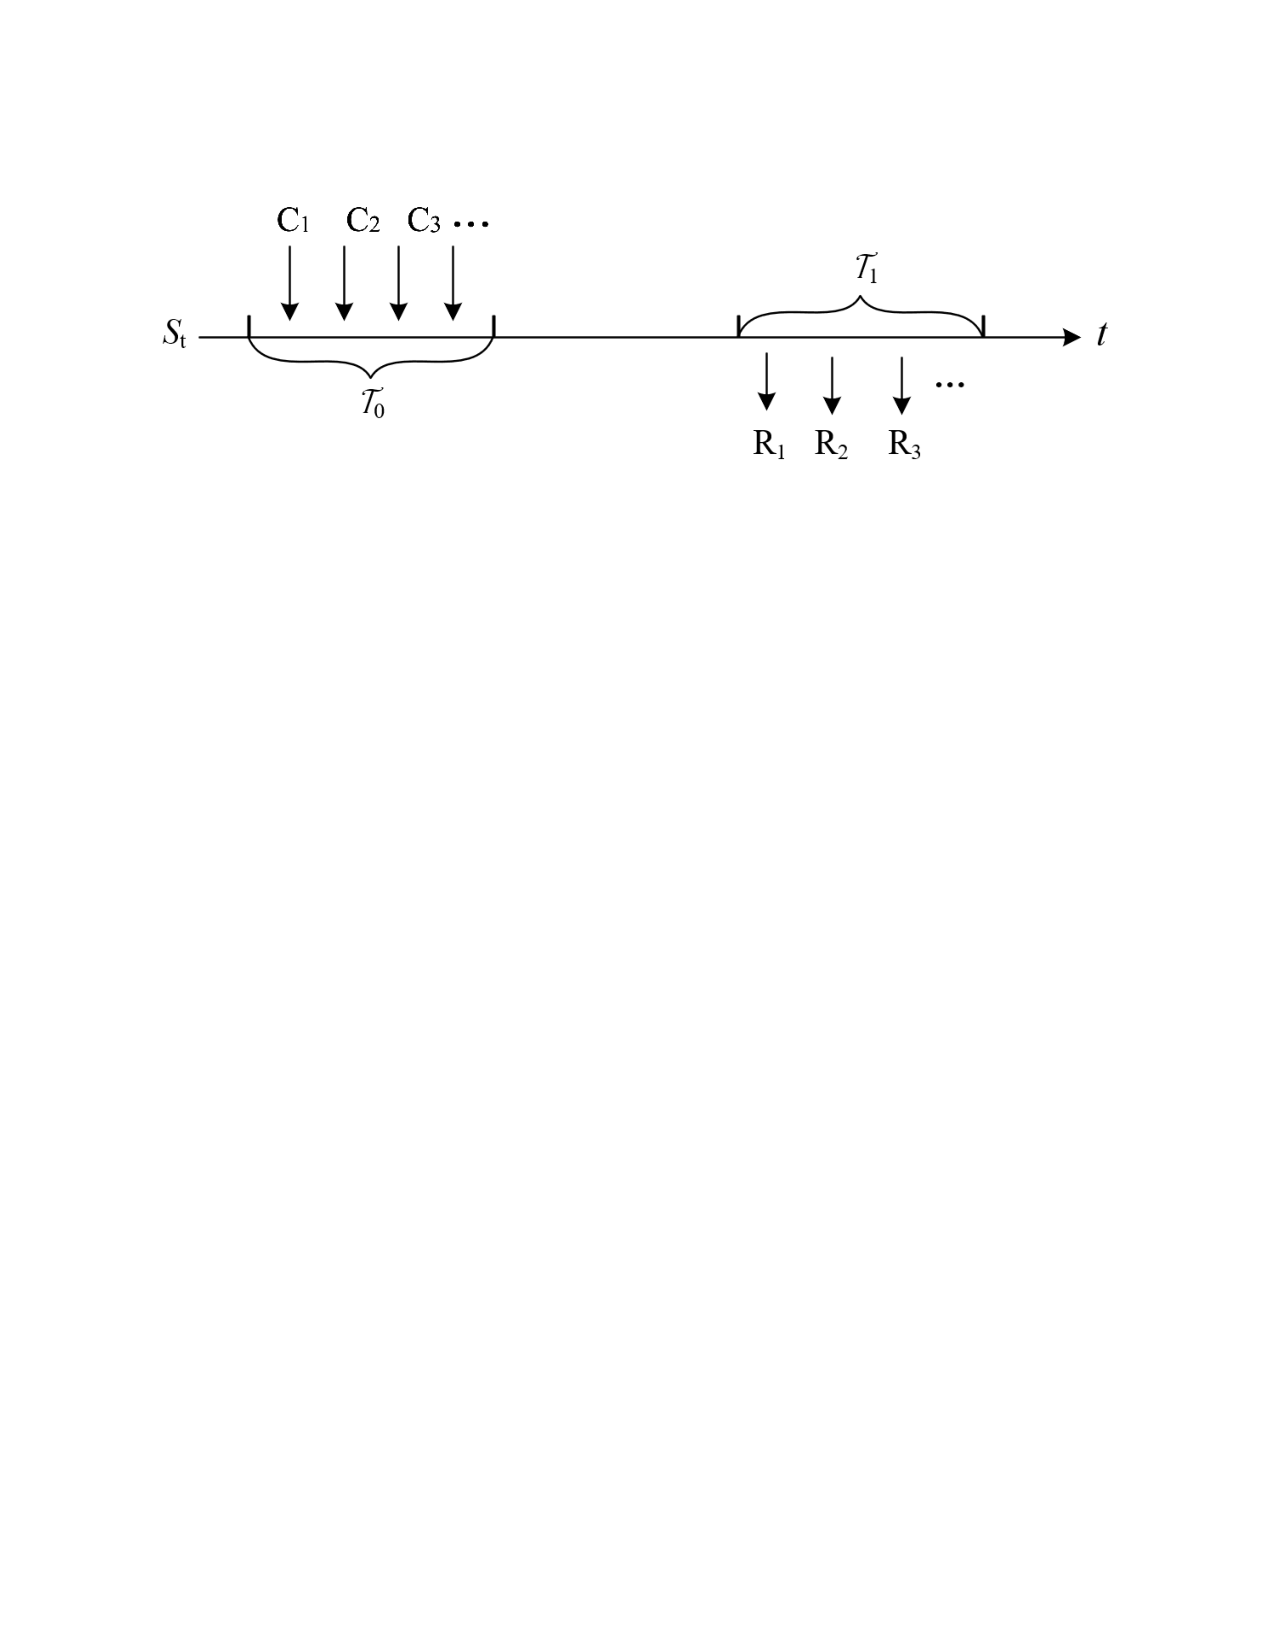
\includegraphics[width=4.5in]{fig-1}
\caption{金融服务或产品的抽象示意图}
\end{figure}

FORT的原理就是,按照给定折现算法,未来收益流和当前支出流等价(或略小,此时为着通缩),因此每一个收益流就对应一个支出流,而收益流和支出流都用统一的去中心化货币单位DCU进行结算。
如果我们把未来收益流称之为金融产品,就可以把对应的支出流称之为产品的现值或成本,这里统一称之为成本,如果我们用$r$表示折现率,$\mathcal{F}_0$代表交易时信息集,这一过程可描述为:

\begin{equation}
\sum_{\mathcal{T}_1} E\left[e^{-rt_{i}}R_{i}|\mathcal{F}_0\right] \leq \sum_{\mathcal{T}_0} E\left[e^{-rt_{i}}C_{i}|\mathcal{F}_0\right] 
\label{e1}
\end{equation}

由于金融产品可以由基础收益函数(简记为BRF)的线性组合构成,每个基础收益函数对应一个折现函数(简记为BDF),这样产品的成本就是这些基本折现函数的线性组合,因此我们可以将基础收益函数及其折现函数设计成一种可开发的模型:折现计算机——任何金融产品都可以由这一计算机开发出来,基础收益函数就像是计算机的指令,基础折现函数就像这些指令的价格或者类似EVM的gas,只不过gas用DCU支付,以及指令会生产出DCU。金融产品$P$及其成本$C(P)$的计算方法可记为:


\begin{equation}
P=x_1\cdot BRF_1+x_2\cdot BRF_2+\cdots=\boldsymbol{BRF}\cdot \boldsymbol{X^T}
\end{equation}

\begin{equation} 
C(P)=x_i\cdot BDF_1+x_2\cdot BDF_2+\cdots=\boldsymbol{BDF}\cdot \boldsymbol{X^T}
\end{equation}

$\boldsymbol{X}$为$P$的$\boldsymbol{BRF}$表示,$\boldsymbol{BDF}$为$\boldsymbol{BRF}$的折现函数,其中:
\begin{equation}
E\left[e^{-rt_{i}}BRF_{i}|\mathcal{F}_0\right] \leq E\left[e^{-rt_{i}}BDF_{i}|\mathcal{F}_0\right] 
\label{eq4}
\end{equation}

基于折现计算机可以开发各种金融产品,包括期权、永续、杠杆交易、互换、 普通交易和借贷等等,几乎所有的金融产品都可以被生产出来。

\subsection{DCU发行结算及定价}
DCU全称是Decentralized Currency Unit,去中心化货币单位,DCU由FORT协议发行,没有上限,初始DCU不超过1亿枚。
在FORT协议里,DCU是唯一的货币单位,你支出用的是DCU,得到的也是DCU。
比如:在未来时刻,符合一定条件的话,你会得到300 DCU,那么你现在需要支出50 DCU,这50 DCU销毁,等到300000区块后,你得到300 DCU,这些DCU是由系统增发出来。

可以看到,所有持有DCU的人共同承担了DCU增发或者销毁的风险和收益, 并且参与DCU的二级市场供给和需求的均衡之中:DCU的需求是那些在链上购买金融产品的人和投资DCU的人,供给则由初始发行量和Fort协议结算出的DCU共同决定,二者在交易所达成价格均衡。
共用同一个计价单位的好处是:我们只需要不断提升 DCU的流动性,就可以解决所有金融服务了,而不需要构建过多的代币,无论是交易、借贷、衍生品都可以通过DCU计价、支付和结算单位来解决。

根据:
\begin{equation}
E\left[e^{-rt}BRF|\mathcal{F}_0\right] \leq E\left[e^{-rt}BDF|\mathcal{F}_0\right] 
\end{equation}

可知总供给$G_t$满足:

\begin{equation} 
EG_{t_2} \leq EG_{t_1}, \quad t_2 \geq t_1 
\end{equation}

DCU总需求($D_t$)由交易需求决定,DCU价格($P_t$)则由$(D_t, G_t)$均衡决定,由于供给的长期期望值逐渐减小,随着FORT得到更多的认可,需求会长期增长,因此$P_t$具备了内在的长期上涨逻辑。

正如DCU的命名,结合FORT合约,它是一个带有场景的链上通用货币,这是BTC和ETH 所不能实现的:BTC没有链上场景,且发行固定,ETH虽然作为gas跟随所有的场景,但其发行是按照固定算法,而不是按照场景增发的。
DCU保证在每个场景里出清,这和之前很多经济学家设想的完全去中心化的货币吻合,是BTC-ETH之后的进一步发展。

\subsection{NEST预言机}
NEST预言机是目前市场上唯一真正去中心化的预言机:给定链外一个价格流,如何设计一个去中心化博弈,使得该博弈均衡能输出一个价格流,并保证该价格流与链外价格流偏差尽可能小。
NEST预言机通过报价挖矿、双向期权、验证周期、价格链及$\beta$系数等模块解决了这一问题,这是一个极其完美的设计。
NEST提供的价格序列,并不改变资产价格的分布,而是接近一种离散的取样模型,这是由去中心化博弈的结构决定的,报价偏差和报价密度取决于套利市 场的深度和NEST token的价格。
总体来说,NEST提供了一个有效的去中心化预言机,保持了价格的基本性状。

在FORT的设计里,我们倾向于使用高度有效的市场价格,因此选择的标的为流动性最好的BTC和ETH等,基本的价格模型为几何布朗运动,即GBM模型。考虑到价格的偏差和离散时间特性,我们会对价格进行GBM下的修正,此为$k$系数修正。
\begin{equation} 
K =(0.00002 * T + 4 * \sigma) * \gamma(\sigma)
\end{equation}

其中$\sigma$为秒级波动率,$T$为时间延迟由打包成功区块高度与最近有效 NEST价格所在区块高度之差乘以区块时间间隔得出,$\gamma$取值满足:
\begin{equation} 
\gamma =\begin{cases}1,\qquad \sigma \leq 0.0003\\
1.5,\quad 0.0003 <\sigma \leq 0.0005\\
2,\qquad \sigma  >0.0005\end{cases}
\end{equation}

\subsection{时间域}
时间域用$\mathcal{T}_i$表示,主要分为时刻和区间,时刻可以是一个确定的时刻,也可以是一个随机的时刻(比如停时),在金融领域,区间往往用来确定某个均值或者停时。
虽然区块链上的时间是离散的,但在一个较长的周期里,可以忽略这些离散的差异,在较短的时间内则可以基于$k$系数进行补偿,因此可以近似用连续时间区间来理解。

\subsection{折现计算机}

我们将所有金融产品(服务)都抽象成了一个收益流和支出流的互换,而收益流由基础收益函数的线性组合表示,那么任何金融产品开发只需要确定基础收益函数的线性组合,就能通过折现函数的线性组合得到其成本(现值),这样一个线性的组合与我们使用计算机编程是一样的,因此我们将这一模块形象称之为折现计算机。
任意金融产品便对应一段计算机编程,这样DeFi的可组合行在这里变成了同一框架的程序设计和程序调用,降低了理解和风险管理难度。

\subsection{基础收益函数与折现函数}

基础收益函数(BRF)可以示确定值(如第13678933区块得到1000DCU),也可以引入NEST预言机价格后成为一个随机变量。
在这里,我们考虑确定值、NEST价格预言机的随机变量、纯概率随机变量等基本类型,每一种类型都由多项式函数域,指数函数、对数函数、绝对值函数、最大最小函数和定积分算子构成,而折现函数(BDF)则包含一个正态分布函数以及多项式函数、指数函数、对数函数等,这里考虑到现实中并不需要那么多的收益函数以及计算复杂性问题,我们选择了一个较为简单的函数列表,后面可以逐渐完善。
如前面所说,基础收益函数就是折现计算机的基础指令,一个金融产品就是一个程序,程序就是这些指令的组合。


\subsection{折现率及利率预言机}
原则上,折现率反应链上世界的无风险回报,我们可以选择一个链上的无风险利率统计量入ETH的PoS收益率或者去中心化利率预言机(一种设计如下:给定每年的DCU发行数量,任何人锁仓DCU就可以参与平分这些发行)提供的利率作为折现率,但这个范式是在传统中心化世界里考虑的,在一个去中心化世界里,为了使得DCU的增发具备通缩属性,从而保证DCU稳定上涨,我们可以将折现率取一个比较小的值,甚至为0。

\subsection{计价单位变换}
如果需要以某种法比或者ETH为计价单位,在FORT里,只需要引入DCU/USDT或者 DCU/ETH价格即可,这一价格可以通过NEST预言机得到。如果DCU的流动性足够大,以至于单一金融产品的结算对价格影响较小,则引入价格的金融产品和传统金融产品无异,基于风险中性测度($E^Q$)的定价可以完美解决折现函数的计算,这类金融产品可以用来做对冲或资产组合管理。
\begin{equation}
E^Q\left[e^{-rt_{i}}BRF_{i}|\mathcal{F}_0\right] \leq E^Q\left[e^{-rt_{i}}BDF_{i}|\mathcal{F}_0\right] 
\end{equation}

\subsection{金融产品开发}

金融产品的开发在这里和写智能合约一样,即对目标的收益找到以BRF为基的一个向量,该向量就代表了这一金融产品,同时该向量与对应的BDF基的乘积就是金融产品的成本,也就是只需要在时间域$\mathcal{T}_0$里支付该成本,就得到了该金融产品。而该金融产品在时间域$\mathcal{T}_1$内会得到FORT合约增发的DCU,其数量就是该向量与BRF的乘积。
这一过程和编写普通智能合约代码一样,就是一个机械的过程。这使得你想要的金融产品都可以用FORT的折现计算机编程实现,具备了统一性,而且开发者不用再去运营代币的流动性,只需要DCU具备足够流动性即可。


\section{应用举例}
FORT的应用范围极为广泛,几乎涵盖了所有金融服务,也包括不同的交易结构(包含点对点,多对多等),同时可以锁定各种链外经济关系,是区块链发展史的一个里程碑式的设计。

\subsection{期权及期权币}
期权发行变得非常简单,只需要输入到期日和执行价格,就得到一个看涨或看跌期权,其成本由折现函数确定,不过在不引用DCU价格的情况下,这一公式并不是风险中性测度的,因此需要注意理解其含义。
如果引用了DCU价格则和传统期权一样,只是交互变得简单得多,没有太多的撮合需要考虑。
一种更好的模型是将期权发行成一种token,即在给定到期日和执行价下,不管从何时开始发行都是同一个代币,这一模型的好处是,可以让传统衍生品交易所不用考虑发行和结算问题:为了满足发行需求,要么需要做大量撮合,要么需要找到做市商,而为了结算,往往需要保证金管理,并且做市商还需要发展出一套对冲策略,这是一个庞大的金融辅助系统,虽然传统金融乐此不彼,但其成本是远高于 FORT模型的,因为用后者发行和结算的话,交易所只需要解决衍生品的二级市场交易问题即可。

\subsection{永续合约、杠杆交易及杠杆币}
永续合约或者杠杆交易也会变得非常简单,这是一个动态结算模型,也是一个基本收益函数,我们也可以将永续或者杠杆交易开发成一种叫做杠杆币的模型:依据价格动态改变其代币的余额,这在当前的算法稳定币也得到过实践。

\subsection{交易、价格币及稳定币}
一个原生资产其实等于一个价格币*DCU计价单位,相当于把一个资产拆分成动态价格和固定的结算单位,只是这种模式只有在完全去中心化世界里能够有效实现:传统中心化世界存在兑付的信用风险。
因此交易就等于用DCU换取各种价格币,或者用各种价格币结算出DCU,或者用原生资产1比1对应价格币(实际上略有偏差,这是价格预言机的偏差导致)。
以此类推,挂靠法币如美元的稳定币就是一个USDT的价格币。

\subsection{指数币和对数币}
一种新的范式是指数币,即价格波动的比例用指数的方式反馈到收益的增长上,与杠杆币相比,指数币拥有良好的性能:永不需要平仓,增长速度更快,可以互相转账,同一地址可以自由叠加等。比如当价格翻一倍时,以e为底的指数 币可以增长 7.4 倍,价格翻2倍时,指数币增长20倍。

\subsection{收益互换}
各种未来的收益互换无非就是成本的交换,因为都等价于未来收益流的折现。

\subsection{借贷}
借贷变得更简单,抵押FORT合约认可的资产,即可获得对应的DCU,偿还即可得到抵押资产,触碰清算线便会被清算,这里的核心参数是清算线、抵押率、利率等。

\subsection{保险}
基于事件的尾部特征,可以制作一种价格保险,将尾部损失与保费互换。

\subsection{利率衍生品}
基于基础利率设计的各种利率衍生品,只需要拥有利率预言机的信息流便可以设计和其价格信息流下类似的各种衍生品。

\subsection{概率币}
设计一种在给定时刻,以某个事先确定的概率得到DCU的代币,如10分之一概率币,每个概率币可以有10分之一的概率得到10个DCU。

\subsection{NFT 应用}
可以基于DCU锁定任何链外游戏或者NFT设计的经济关系,即所有的游戏资产可以对应某种概率币或者以上某种衍生品。
这样无论是在哪个游戏里,其游戏资产对应的 NFT可以在FORT里被兑付,无论该游戏是否存在,从而构建了游戏世界的一致性变量。

\subsection{多向交易}
设计一种两个或多个参与者的交易:A和B可以基于FORT制定一种合约,在当前时刻各支付一定的DCU,并在未来得到对应的DCU,这样FORT可以参与到二者的分配之中,从而实现一种多人竞争和博弈的结构。

\section{总结}
FORT提供了一种全新的范式:将金融产品理解成基本折现函数的编程,其成本便是调用该函数的费用,这和EVM很类似,不同的是,折现计算机的经济关系是内生的。
这种新的范式可以覆盖几乎所有的金融产品(服务),并且随时可以买入并无限流动性结算,这里不需要做市商,不需要保证金,不需要追缴保证金(Margin Call),不用担心无法结算。
只要DCU的流动性足够,还原传统金融市场也是极其简单的事情,其功能将十分强大。
而且,由于发行和结算这样的困难问题得到解决,传统衍生品交易所即可专注于二级市场,从而极大降低其成本。
另外,FORT也可以成为构建时下流行的元宇宙的基本一致性变量,具有穿越不同游戏锁定经 济关系的能力,其前景十分广阔。


\bibliography{ref}

\end{document}
